\chapter[Generalized systems]{Generalized systems governing probability density functions
\label{general}}

So far we have considered one-dimensional and two-dimensional release processes. When the
channel can take on two states---open or closed---we have seen that the
associated probability density functions are governed by $2\times2$ systems of
partial differential equations. When a drug is added to the Markov model, an
extra state is introduced associated with either the open or the closed state 
and we obtain a model for the probability density functions phrased in terms of 
$3\times3$ systems of partial differential equations. In subsequent 
chapters, we will study situations involving many states and, to do so 
without drowning in cumbersome notation, we need mathematical formalism to 
present such models compactly. The compact form we use here is taken 
from Huertas and Smith \cite{Huertas2007}. We will introduce the more compact
notation simply by providing a couple of examples. These will,
hopefully, clarify how to formulate rather complex models in an expedient manner.

\bigskip
\section{Two-dimensional calcium release revisited}

Let us start by recalling that the two-dimensional process of calcium release
illustrated in Figure \ref{geom2D} on page \pageref{geom2D} can be modeled as
\begin{align}
\bar{x}^{\prime}(t)  &  =\bar{\gamma}(t)v_{r}\left(  \bar{y}-\bar{x}\right)
+v_{d}\left(  c_{0}-\bar{x}\right)  ,\label{c1g}\\
\bar{y}^{\prime}(t)  &  =\bar{\gamma}(t)v_{r}\left(  \bar{x}-\bar{y}\right)
+v_{s}\left(  c_{1}-\bar{y}\right)  , \label{c2g}%
\end{align}
where $\bar{\gamma}=\bar{\gamma}(t)$ is a stochastic variable governed by a
Markov model represented by a reaction scheme of the form%
\[
C\underset{k_{co}}{\overset{k_{oc}}{\leftrightarrows}}O.
\]
We have seen (see, e.g., page \pageref{eq:pdf21}) that the probability density
functions of the open state $(\rho_{o})$ and the closed state $(\rho_{c})$ are
governed by the system
\begin{align}
\frac{\partial\rho_{o}}{\partial t}+\frac{\partial}{\partial x}\left(
a_{o}^{x}\rho_{o}\right)  +\frac{\partial}{\partial y}\left(  a_{o}^{y}%
\rho_{o}\right)   &  =k_{co}\rho_{c}-k_{oc}\rho_{o},\label{eq:pdf21g}\\
\frac{\partial\rho_{c}}{\partial t}+\frac{\partial}{\partial x}\left(
a_{c}^{x}\rho_{c}\right)  +\frac{\partial}{\partial y}\left(  a_{c}^{y}%
\rho_{c}\right)   &  =k_{oc}\rho_{o}-k_{co}\rho_{c}, \label{eq:pdf22g}%
\end{align}
where
\begin{align}
a_{o}^{x}  &  =v_{r}\left(  y-x\right)  +v_{d}\left(  c_{0}-x\right)
,\nonumber\\
a_{o}^{y}  &  =v_{r}\left(  x-y\right)  +v_{s}\left(  c_{1}-y\right)
,\label{eq:fluxes2Dg}\\
a_{c}^{x}  &  =v_{d}\left(  c_{0}-x\right)  ,\nonumber\\
a_{c}^{y}  &  =v_{s}\left(  c_{1}-y\right)  .\nonumber
\end{align}
To prepare ourselves for more complex systems, we number the states
in this simple system with $i=1,2,$ where $i=1$ is for the open state and $i=2$ is for the closed state. The
system can now be written in the form%

\[
\frac{\partial\rho_{i}}{\partial t}+\frac{\partial}{\partial x}\left(
a_{i}^{x}\rho_{i}\right)  +\frac{\partial}{\partial y}\left(  a_{i}^{y}%
\rho_{i}\right)  =\left(  K\rho\right)  _{i},
\]
where $\left(  K\rho\right)  _{i}$ denotes the $i$th component of the matrix
vector product $K\rho.$ Here the vector $\rho$ is given by%
\[
\rho=\left(
\begin{array}
[c]{c}%
\rho_{1}\\
\rho_{2}%
\end{array}
\right)  =\left(
\begin{array}
[c]{c}%
\rho_{o}\\
\rho_{c}%
\end{array}
\right)  
\]
and the matrix is given by%
\[
K=\left(
\begin{array}
[c]{cc}%
-k_{12} & k_{21}\\
k_{12} & -k_{21}%
\end{array}
\right) =\left(
\begin{array}
[c]{cc}%
-k_{oc} & k_{co}\\
k_{oc} & -k_{co}%
\end{array}
\right) .
\]
Furthermore, we introduce the functions%
\begin{align*}
a_{i}^{x}  &  =\gamma_{i}v_{r}\left(  y-x\right)  +v_{d}\left(  c_{0}%
-x\right)  ,\\
a_{i}^{y}  &  =\gamma_{i}v_{r}\left(  x-y\right)  +v_{s}\left(  c_{1}%
-y\right)  ,
\end{align*}
where $\gamma_{i}$ is one for the open state (i.e., $i=1$) and zero for the closed
state (i.e., $i=2$).
\bigskip

\section{Four-state model}

It useful to illustrate this compact notation for a slightly more complex
model based on four states. Suppose that the Markov model governing the
stochastic variable $\bar{\gamma}$ in model $(\ref{c1g})$ and $(\ref{c2g})$ is
based on four states: two open states $O_{1}$ and $O_{2}$ and two closed
states $C_{1}$ and $C_{2}$, as shown in Figure \ref{M44}.%
\begin{figure}[ptb]
\begin{center}
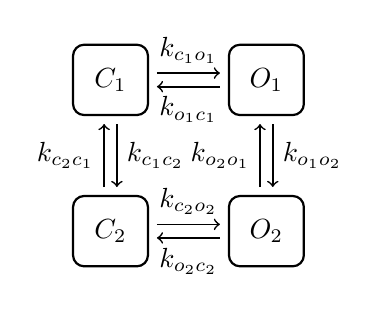
\begin{tikzpicture}[
   font=\sffamily,
   every matrix/.style={ampersand replacement=\&,column sep=1cm,row sep=1cm},
   state/.style={draw,thick,rounded corners,inner sep=.3cm},
   to/.style={->,semithick,shorten >=0.1cm,shorten <=0.1cm},
   Q/.style={->,semithick,sloped,pos=0.700000,shorten >=0.1cm,shorten <=0.1cm},  
   every node/.style={auto}]
\matrix{
\node[state] (C_{1}) {\parbox{10pt}{\centerline{$C_{1}$}}};\&\node[state] (O_{1}) {\parbox{10pt}{\centerline{$O_{1}$}}};\\
\node[state] (C_{2}) {\parbox{10pt}{\centerline{$C_{2}$}}};\&\node[state] (O_{2}) {\parbox{10pt}{\centerline{$O_{2}$}}};\\
};
\draw[to]  (C_{1}.10) to node {$k_{c_{1}o_{1}}$} (O_{1}.170);
\draw[to]  (C_{1}.280) to node {$k_{c_{1}c_{2}}$} (C_{2}.80);
\draw[to]  (O_{1}.190) to node {$k_{o_{1}c_{1}}$} (C_{1}.350);
\draw[to]  (O_{1}.280) to node {$k_{o_{1}o_{2}}$} (O_{2}.80);
\draw[to]  (C_{2}.100) to node {$k_{c_{2}c_{1}}$} (C_{1}.260);
\draw[to]  (C_{2}.10) to node {$k_{c_{2}o_{2}}$} (O_{2}.170);
\draw[to]  (O_{2}.100) to node {$k_{o_{2}o_{1}}$} (O_{1}.260);
\draw[to]  (O_{2}.190) to node {$k_{o_{2}c_{2}}$} (C_{2}.350);
\end{tikzpicture}
\end{center}
\caption{Markov model including four possible states: two open states, $O_{1}$ 
and $O_{2}$, and two closed states, $C_{1}$ and $C_{2}$.}%
\label{M44}%
\end{figure}

The probability density system associated with the model $(\ref{c1g})$ and $(\ref{c2g})$ when the Markov model is given by Figure \ref{M44} can now be 
written in the form%

\begin{align}
\frac{\partial\rho_{o_{1}}}{\partial t}+\frac{\partial}{\partial x}\left(
a_{o}^{x}\rho_{o_{1}}\right)  +\frac{\partial}{\partial y}\left(  a_{o}%
^{y}\rho_{o_{1}}\right)   &  =k_{c_{1}o_{1}}\rho_{c_{1}}-\left(  k_{o_{1}%
c_{1}}+k_{o_{1}o_{2}}\right)  \rho_{o_{1}}+k_{o_{2}o_{1}}\rho_{o_{2}%
},\nonumber\\
\frac{\partial\rho_{o_{2}}}{\partial t}+\frac{\partial}{\partial x}\left(
a_{o}^{x}\rho_{o_{2}}\right)  +\frac{\partial}{\partial y}\left(  a_{o}%
^{y}\rho_{o_{2}}\right)   &  =k_{c_{2}o_{2}}\rho_{c_{2}}-\left(  k_{o_{2}c_{2}%
}+k_{o_{2}o_{1}}\right)  \rho_{o_{2}}+k_{o_{1}o_{2}}\rho_{o_{1}}%
,\label{pdf44}\\
\frac{\partial\rho_{c_{1}}}{\partial t}+\frac{\partial}{\partial x}\left(
a_{c}^{x}\rho_{c_{1}}\right)  +\frac{\partial}{\partial y}\left(  a_{c}%
^{y}\rho_{c_{1}}\right)   &  =k_{o_{1}c_{1}}\rho_{o_{1}}-\left(  k_{c_{1}%
o_{1}}+k_{c_{1}c_{2}}\right)  \rho_{c_{1}}+k_{c_{2}c_{1}}\rho_{c_{2}%
},\nonumber\\
\frac{\partial\rho_{c_{2}}}{\partial t}+\frac{\partial}{\partial x}\left(
a_{c}^{x}\rho_{c_{2}}\right)  +\frac{\partial}{\partial y}\left(  a_{c}%
^{y}\rho_{c_{2}}\right)   &  =k_{c_{1}c_{2}}\rho_{c_{1}}-\left(  k_{c_{2}%
c_{1}}+k_{c_{2}o_{2}}\right)  \rho_{c_{2}}+k_{o_{2}c_{2}}\rho_{o_{2}%
},\nonumber
\end{align}
where %
\begin{align}
a_{o}^{x} &  =v_{r}\left(  y-x\right)  +v_{d}\left(  c_{0}-x\right)
,\nonumber\\
a_{o}^{y} &  =v_{r}\left(  x-y\right)  +v_{s}\left(  c_{1}-y\right)
,\label{flux44}\\
a_{c}^{x} &  =v_{d}\left(  c_{0}-x\right)  ,\nonumber\\
a_{c}^{y} &  =v_{s}\left(  c_{1}-y\right)  .\nonumber
\end{align}
By defining the states $O_{1},O_{2},C_{1},$ and $C_{2}$ to be the states 
1, 2, 3, and
4, respectively, we can write the system $(\ref{pdf44})$ in the more compact form%
\begin{equation}
\frac{\partial\rho_{i}}{\partial t}+\frac{\partial}{\partial x}\left(
a_{i}^{x}\rho_{i}\right)  +\frac{\partial}{\partial y}\left(  a_{i}^{y}%
\rho_{i}\right)  =\left(  K\rho\right)  _{i}\label{compact44}%
\end{equation}
for $i=1,2,3,4,$ where%
\begin{align*}
a_{i}^{x} &  =\gamma_{i}v_{r}\left(  y-x\right)  +v_{d}\left(  c_{0}-x\right)
,\\
a_{i}^{y} &  =\gamma_{i}v_{r}\left(  x-y\right)  +v_{s}\left(  c_{1}-y\right),
\end{align*}
and $\rho=(\rho_1,\rho_2,\rho_3,\rho_4)^T.$ 
Here $\gamma_{i}$ is one for the open states (i.e., $i=1$ and $i=2$) and zero for
the closed states (i.e., $i=3$ and $i=4$). Furthermore, the matrix is given by%
\[
K=\left(
\begin{array}
[c]{cccc}%
-\left(  k_{o_{1}c_{1}}+k_{o_{1}o_{2}}\right)   & k_{o_{2}o_{1}} &
k_{c_{1}o_{1}} & 0\\
k_{o_{1}o_{2}} & -\left(  k_{o_{2}c_{2}}+k_{o_{2}o_{1}}\right)   & 0 &
k_{c_{2}o_{2}}\\
k_{o_{1}c_{1}} & 0 & -\left(  k_{c_{1}o_{1}}+k_{c_{1}c_{2}}\right)   &
k_{c_{2}c_{1}}\\
0 & k_{o_{2}c_{2}} & k_{c_{1}c_{2}} & -\left(  k_{c_{2}c_{1}}+k_{c_{2}o_{2}%
}\right)
\end{array}
\right),
\]
which in compact notation is%
\[
K=\left(
\begin{array}
[c]{cccc}%
-\left(  k_{13}+k_{12}\right)   & k_{21} & k_{31} & 0\\
k_{12} & -\left(  k_{24}+k_{21}\right)   & 0 & k_{42}\\
k_{13} & 0 & -\left(  k_{31}+k_{34}\right)   & k_{43}\\
0 & k_{24} & k_{34} & -\left(  k_{43}+k_{42}\right)
\end{array}
\right)  .
\]

\bigskip
\section{Nine-state model}

We have seen how to formulate probability density systems for two-state and
four-state Markov models.  For even larger Markov models, it is useful to
introduce two-dimensional numbering. This will be illustrated using the nine-state model 
given in Figure \ref{ninestates}.%
\begin{figure}[ptb]
\begin{center}
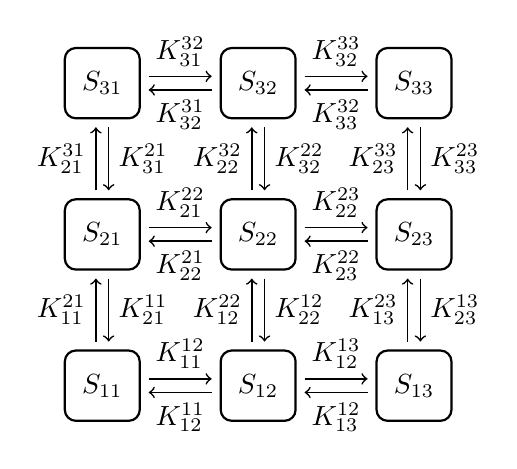
\begin{tikzpicture}[
   font=\sffamily,
   every matrix/.style={ampersand replacement=\&,column sep=1cm,row sep=1cm},
   state/.style={draw,thick,rounded corners,inner sep=.3cm},
   to/.style={->,semithick,shorten >=0.1cm,shorten <=0.1cm},
   Q/.style={->,semithick,sloped,pos=0.700000,shorten >=0.1cm,shorten <=0.1cm},  
   every node/.style={auto}]
\matrix{
\node[state] (S_{31}) {\parbox{10pt}{\centerline{$S_{31}$}}};\&\node[state] (S_{32}) {\parbox{10pt}{\centerline{$S_{32}$}}};\&\node[state] (S_{33}) {\parbox{10pt}{\centerline{$S_{33}$}}};\\
\node[state] (S_{21}) {\parbox{10pt}{\centerline{$S_{21}$}}};\&\node[state] (S_{22}) {\parbox{10pt}{\centerline{$S_{22}$}}};\&\node[state] (S_{23}) {\parbox{10pt}{\centerline{$S_{23}$}}};\\
\node[state] (S_{11}) {\parbox{10pt}{\centerline{$S_{11}$}}};\&\node[state] (S_{12}) {\parbox{10pt}{\centerline{$S_{12}$}}};\&\node[state] (S_{13}) {\parbox{10pt}{\centerline{$S_{13}$}}};\\
};
\draw[to]  (S_{31}.10) to node {$K_{31}^{32}$} (S_{32}.170);
\draw[to]  (S_{31}.280) to node {$K_{31}^{21}$} (S_{21}.80);
\draw[to]  (S_{32}.190) to node {$K_{32}^{31}$} (S_{31}.350);
\draw[to]  (S_{32}.10) to node {$K_{32}^{33}$} (S_{33}.170);
\draw[to]  (S_{32}.280) to node {$K_{32}^{22}$} (S_{22}.80);
\draw[to]  (S_{33}.190) to node {$K_{33}^{32}$} (S_{32}.350);
\draw[to]  (S_{33}.280) to node {$K_{33}^{23}$} (S_{23}.80);
\draw[to]  (S_{21}.100) to node {$K_{21}^{31}$} (S_{31}.260);
\draw[to]  (S_{21}.10) to node {$K_{21}^{22}$} (S_{22}.170);
\draw[to]  (S_{21}.280) to node {$K_{21}^{11}$} (S_{11}.80);
\draw[to]  (S_{22}.100) to node {$K_{22}^{32}$} (S_{32}.260);
\draw[to]  (S_{22}.190) to node {$K_{22}^{21}$} (S_{21}.350);
\draw[to]  (S_{22}.10) to node {$K_{22}^{23}$} (S_{23}.170);
\draw[to]  (S_{22}.280) to node {$K_{22}^{12}$} (S_{12}.80);
\draw[to]  (S_{23}.100) to node {$K_{23}^{33}$} (S_{33}.260);
\draw[to]  (S_{23}.190) to node {$K_{23}^{22}$} (S_{22}.350);
\draw[to]  (S_{23}.280) to node {$K_{23}^{13}$} (S_{13}.80);
\draw[to]  (S_{11}.100) to node {$K_{11}^{21}$} (S_{21}.260);
\draw[to]  (S_{11}.10) to node {$K_{11}^{12}$} (S_{12}.170);
\draw[to]  (S_{12}.100) to node {$K_{12}^{22}$} (S_{22}.260);
\draw[to]  (S_{12}.190) to node {$K_{12}^{11}$} (S_{11}.350);
\draw[to]  (S_{12}.10) to node {$K_{12}^{13}$} (S_{13}.170);
\draw[to]  (S_{13}.100) to node {$K_{13}^{23}$} (S_{23}.260);
\draw[to]  (S_{13}.190) to node {$K_{13}^{12}$} (S_{12}.350);
\end{tikzpicture}
\end{center}
\caption{Markov model including nine possible states.}%
\label{ninestates}%
\end{figure}
Here $S_{ij},$ $i,j=1,2,3$, denotes the states of the Markov model and
$K_{ij}^{mn}$ denotes\footnote{We use $K_{ij}$ as shorthand for $K_{i,j},$ but
we use the comma when an index of the form $j+1$ is needed, that is we write
$K_{i,j+1}.$} the reaction rate from the state $S_{ij}$ to the state $S_{mn}.$
The system governing the probability density functions of these states can be
written in the form%
\begin{equation}
\frac{\partial\rho_{ij}}{\partial t}+\frac{\partial}{\partial x}\left(
a_{ij}^{x}\rho_{ij}\right)  +\frac{\partial}{\partial y}\left(  a_{ij}^{y}%
\rho_{ij}\right)  =R_{ij},\label{pdf99}%
\end{equation}
where%
\begin{align*}
R_{ij}  & =K_{i,j+1}^{i,j}\rho_{i,j+1}+K_{i+1,j}^{i,j}\rho_{i+1,j}%
+K_{i,j-1}^{i,j}\rho_{i,j-1}+K_{i-1,j}^{i,j}\rho_{i-1,j}\\
& -\left(  K_{i,j}^{i,j+1}+K_{i,j}^{i+1,j}+K_{i,j}^{i,j-1}+K_{i,j}%
^{i-1,j}\right)  \rho_{i,j}.
\end{align*}
Here $\rho_{ij}$ denotes the probability density function of the state
$S_{ij}$ and we use the convention that $K_{ij}^{mn}=0$ for $i,j,m,n\notin%
\left\{  1,2,3\right\}  .$ We also have%
\begin{align*}
a_{ij}^{x} &  =\gamma_{ij}v_{r}\left(  y-x\right)  +v_{d}\left(
c_{0}-x\right)  ,\\
a_{ij}^{y} &  =\gamma_{ij}v_{r}\left(  x-y\right)  +v_{s}\left(
c_{1}-y\right)  ,
\end{align*}
where $\gamma_{ij}=1$ when the state $S_{ij}$ represents an open state and
$\gamma_{ij}=0$ when $S_{ij}$ represents a closed state.



